\section{Prelimenaries}
\label{sec:pre}

% Kartik 11/13 start
We introduce the core notation and concepts used in our causal preference framework: the Med-LVLM formulation, preference optimization, and causal counterfactual learning.

A Med-LVLM combines a visual encoder with an LLM to process multimodal medical inputs. Given a medical image $I$ and a clinical query $T$, the input is $x=(I,T)$, and the model predicts autoregressively predicts next token probabilities $\pi_\theta(y_i|y_{<i},x)$, yielding sequence likelyhood $\pi_\theta(y|x) = \prod_i \pi_\theta(y_i|y_{<i},x)$, where $y$ is the generated medical report or answer.

\textbf{Preference Optimization.}
Preference optimization aligns the conditional policy using pairwise preference supervision, $x, y_{\omega},y_l$. DPO \cite{rafailov2023direct} directly connects policy with the reward difference between preferred and dispreferred responses. To remove the explicit reward model, DPO reformulates this closed-form expression as a supervised learning objective. Given a preference dataset $\mathcal{D}=\{(x^{(i)},y_w^{(i)},y_l^{(i)})\}_{i=1}^{N}$, where $y_w$ and $y_l$ denote the preferred and dispreferred responses for input $x$, the DPO loss is
\begin{equation}
\small
\begin{aligned}
&\mathcal{L}_{\text{DPO}}(\pi_\theta; \pi_{\text{ref}}) 
= -\mathbb{E}_{(x,y_w,y_l)\sim\mathcal{D}} \\&\Bigg[
\log \sigma \Big(
\eta^{-1} \log \frac{\pi_\theta(y_w|x)}{\pi_{\text{ref}}(y_w|x)}
- \eta^{-1} \log \frac{\pi_\theta(y_l|x)}{\pi_{\text{ref}}(y_l|x)}
\Big) \Bigg].
\end{aligned}
\label{eq:dpo_loss}
\end{equation} 
We provide the complete derivation in Appendix~\ref{supp:pref_optim}.

\begin{figure}[t]
    \centering
    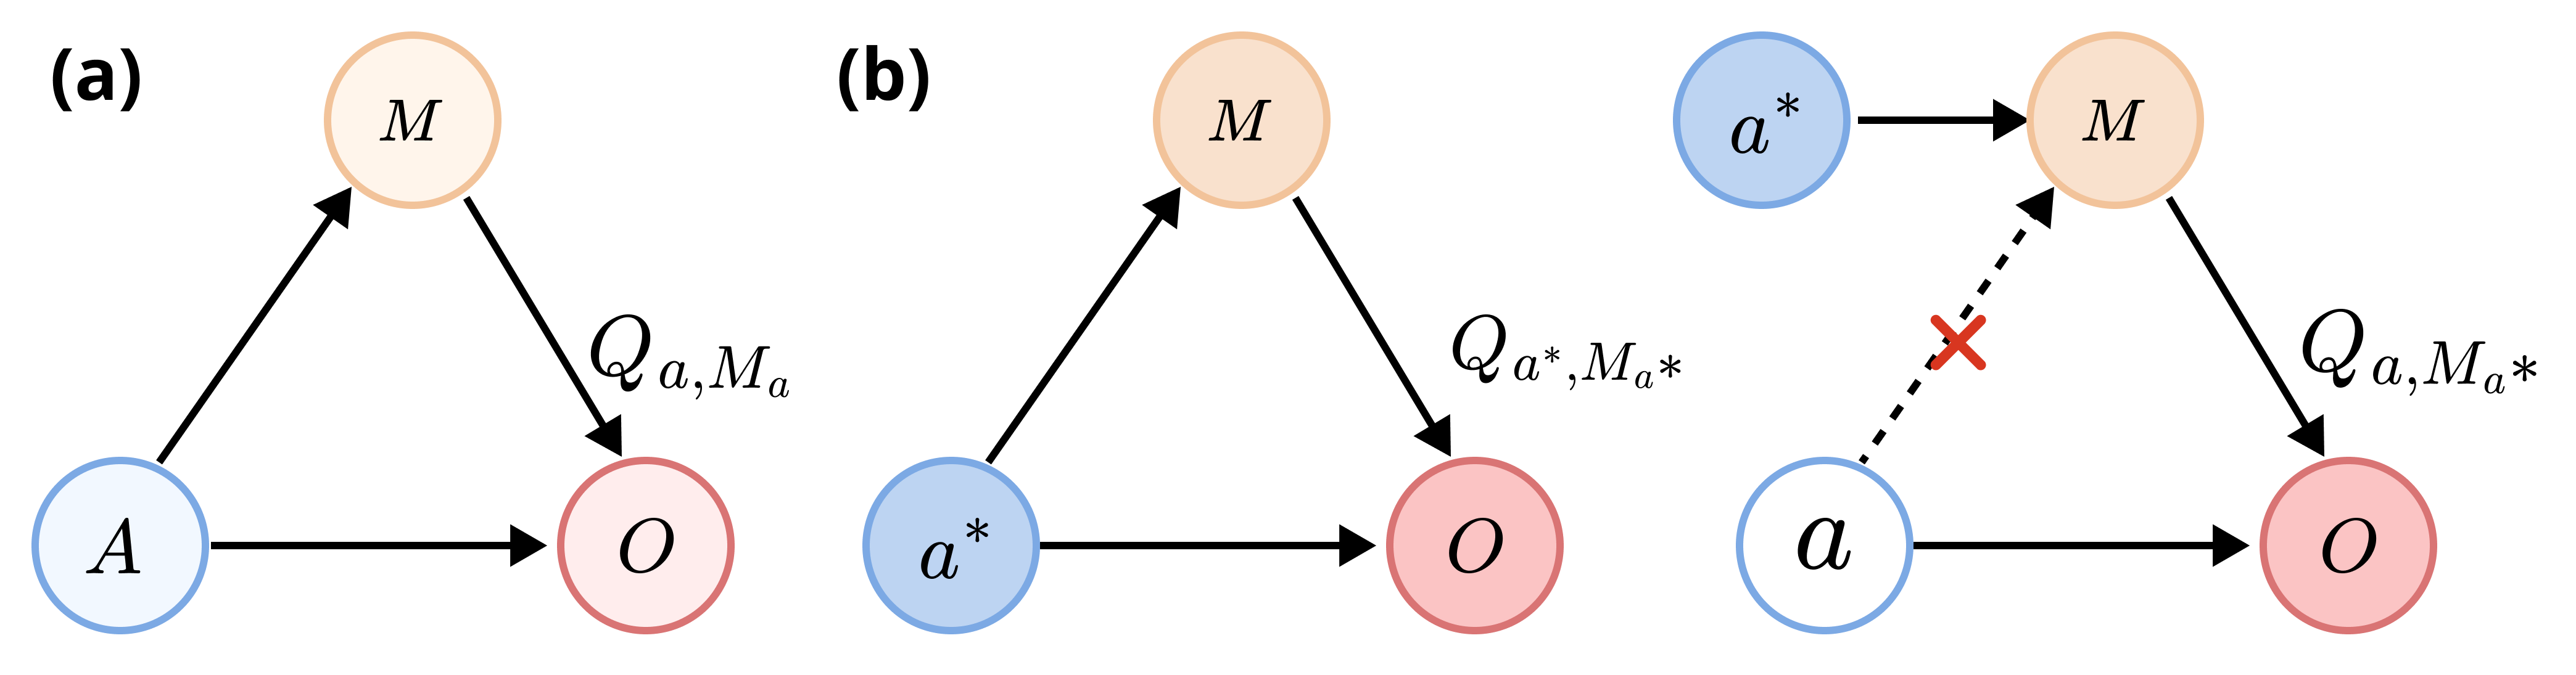
\includegraphics[width=0.45\textwidth]{figs/cvpr_fig2.png}
    \caption{ (a) Example of causal graph. (b) Examples of counterfactual notations.}
    \label{fig:c1}
\end{figure}

\textbf{Causal Counterfactual Learning.} Causal counterfactual learning formalizes how outcomes change under hypothetical interventions using structural causal models (SCMs) \cite{pearl2009causality}. We define a causal graph $\mathcal{G}=\{\mathcal{V}, \mathcal{E}\}$, where $\mathcal{V}$ and $\mathcal{E}$ denote the sets of variables and directed edges, respectively. As shown in Fig. \ref{fig:c1}, for a causal chain $A \!\to\! M \!\to\! O$ $A$ denotes the \textit{cause}, $M$ represents the \textit{mediator},  and $O$ is the \textit{effect} or \textit{outcome}. The counterfactual outcome, $O_{a,m}$ represents the value that $O$ would take if $A$ were set to $a$ and $M$ were set to $m$, i.e., $O_{a,m} = O(A{=}a, M{=}m)$. 

In the factual world, $M=M_a$ and the observed outcome is $B_{a,M_a}$. In the counterfactual world, $A$ may take a different hypothetical value $a^*$, while the mediator is fixed to its factual value $M_a$, yielding $O_{a^*,M_a}$. Causal effects quantify the expected outcome difference between two treatment settings $A=a$ and $A=a^*$. According to the causal theory \cite{pearl2014interpretation}, the Total Effect (TE) of $A$ on $B$ is defined as
\begin{equation}
\text{TE} = O_{a,M_a} - O_{a^*,M_{a^*}},
\end{equation}which decomposes into the Natural Direct Effect (NDE) 
\begin{equation}
\text{NDE} = O_{a,M_{a^*}} - O_{a^*,M_{a^*}},
\end{equation}
and the Total Indirect Effect (TIE) 
\begin{equation}
\text{TIE} = \text{TE} - \text{NDE} = O_{a,M_a} - O_{a,M_{a^*}}.
\end{equation}
where $M_{a^*}$ denotes the value of $M$ had $A$ been $a^*$\cite{pearl2016causal}. NDE isolates the direct causal pathfrom $A$ to $O$ while blocking $M$, whereas TIE captures the mediated contribution through $M$.

% Kartik 11/13 end










%%% OLD VERSION

\iffalse
To facilitate understanding of our causal framework, this section introduces the basic concepts and notation used throughout the paper. We first define the setting of Med-LVLMs and their multimodal representations, followed by two theoretical foundations: preference optimization and causal counterfactual learning.

A Med-LVLM integrates a visual encoder with a large language model (LLM) to process multimodal medical inputs. Given a medical image $I$ and a clinical query $T$ (e.g., a question or report prompt), the combined input is represented as $x = (I, T)$. The model autoregressively predicts the probability distribution of the next token conditioned on the multimodal input, denoted as $\pi_\theta(y_i|y_{<i},x)$. Consequently, the overall conditional likelihood of the generated sequence is expressed as $\pi_\theta(y|x) = \prod_i \pi_\theta(y_i|y_{<i},x)$, where $y$ represents the generated medical report or answer.

\subsection{Preference Optimization}

Building upon the probabilistic formulation introduced above, preference optimization aims to align the conditional policy $\pi_{\theta}(y|x)$ with desired responses based on pairwise preference supervision. 
This paradigm originates from reinforcement learning from human feedback (RLHF) \cite{Christiano2017RLHF}, 
where a reward model $r(x,y)$ is learned to reflect human preference and the policy is optimized with reinforcement learning algorithms such as PPO \cite{Schulman2017PPO}. 
Following the Bradley--Terry model \cite{Bradley1952BT}, the probability of preferring one response $y$ over another $y'$ given the same input $x$ is modeled as
$
P(y \succ y'|x) = \sigma(r(x,y) - r(x,y')) ,
$
where $\sigma(\cdot)$ denotes the sigmoid function. 
Given the true reward model $r(x,y)$, RLHF seeks to maximize the expected reward while constraining deviation from a reference policy $\pi_{\text{ref}}$, formulated as $
\max_{\theta} \; \mathbb{E}_{x,y\sim\pi_\theta} [r(x,y)] - \eta^{-1} \, \mathbb{E}_{x} [\mathrm{KL}(\pi_\theta(\cdot|x) \| \pi_{\text{ref}}(\cdot|x))],
$
where $\eta$ controls the trade-off between reward maximization and policy regularization. 


Rafailov \textit{et al.} \cite{rafailov2023direct} showed that this optimization admits a closed-form solution $
\pi^{*}(y|x) \propto \pi_{\text{ref}}(y|x)\exp(\eta\, r(x,y))$,
which directly connects policy improvement with the reward difference between preferred and dispreferred responses. To remove the explicit reward model, DPO reformulates this closed-form expression as a supervised learning objective. 
Given a preference dataset $\mathcal{D}=\{(x^{(i)},y_w^{(i)},y_l^{(i)})\}_{i=1}^{N}$, where $y_w$ and $y_l$ denote the preferred and dispreferred responses for input $x$, the DPO loss is
\begin{equation}
\small
\begin{aligned}
&\mathcal{L}_{\text{DPO}}(\pi_\theta; \pi_{\text{ref}}) 
= -\mathbb{E}_{(x,y_w,y_l)\sim\mathcal{D}} \\&\Bigg[
\log \sigma \Big(
\eta^{-1} \log \frac{\pi_\theta(y_w|x)}{\pi_{\text{ref}}(y_w|x)}
- \eta^{-1} \log \frac{\pi_\theta(y_l|x)}{\pi_{\text{ref}}(y_l|x)}
\Big) \Bigg].
\end{aligned}
\label{eq:dpo_loss}
\end{equation}
This formulation directly calibrates the relative log-likelihood between preferred and dispreferred responses, providing a stable and reward-free approach for preference-based alignment of large multimodal models.

\subsection{Causal Counterfactual Learning}

Causal counterfactual learning provides a principled framework for analyzing how outcomes would change under hypothetical interventions. 
Following the structural causal model (SCM) framework \cite{pearl2009causality}, 
we define a causal graph $\mathcal{G}=\{\mathcal{V}, \mathcal{E}\}$, where $\mathcal{V}$ and $\mathcal{E}$ denote the sets of variables and directed edges, respectively. 
In our setting, $A$ denotes the \textit{cause}, 
$M$ represents the \textit{mediator}, 
and $O$ is the \textit{effect} or \textit{outcome}.
The typical causal structure can be represented as $A \!\to\! M \!\to\! O$.  

\noindent\textbf{Counterfactual Notations.} Counterfactual notation is used to formalize causal assumptions derived from $\mathcal{G}$. The term $O_{a,m}$ represents the value that $O$ would take if $A$ were set to $a$ and $M$ were set to $m$, i.e., $O_{a,m} = O(A{=}a, M{=}m)$. 
In the factual world, $M=M_a$ and the observed outcome is $B_{a,M_a}$. In the counterfactual world, $A$ may take a different hypothetical value $a^*$, while the mediator is fixed to its factual value $M_a$, yielding $O_{a^*,M_a}$. 

\noindent\textbf{Causal Effects.} Causal effects quantify the expected outcome difference between two treatment settings $A=a$ and $A=a^*$. According to the causal theory \cite{pearl2014interpretation}, the Total Effect (TE) of $A$ on $B$ is defined as
\begin{equation}
\text{TE} = O_{a,M_a} - O_{a^*,M_{a^*}}.
\end{equation}
It can be decomposed into the Natural Direct Effect (NDE) and the Total Indirect Effect (TIE) \cite{pearl2016causal}. 
The NDE isolates the direct path from $A$ to $O$ while blocking $M$:
\begin{equation}
\text{NDE} = O_{a,M_{a^*}} - O_{a^*,M_{a^*}},
\end{equation}
where $M_{a^*}$ denotes the value of $M$ had $A$ been $a^*$. 
The TIE captures the effect transmitted through the mediator:
\begin{equation}
\text{TIE} = \text{TE} - \text{NDE} = O_{a,M_a} - O_{a,M_{a^*}}.
\end{equation}
These decompositions provide a principled way to separate the direct causal influence of biased factors from the mediated effects that encode valuable clinical information.

\fi